\renewcommand{\theequation}{\theenumi}
\begin{enumerate}[label=\thesection.\arabic*.,ref=\thesection.\theenumi]
\numberwithin{equation}{enumi}

\begin{figure}[!ht]
\centering
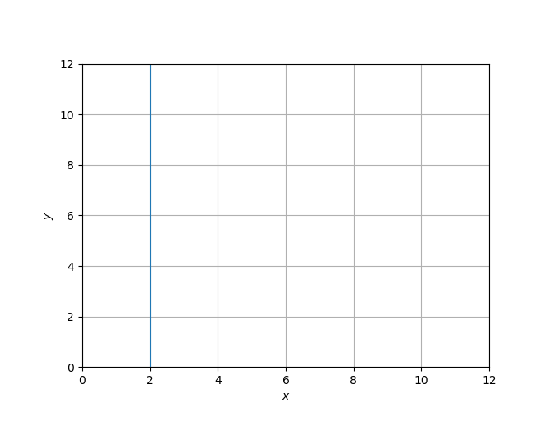
\includegraphics[width= \columnwidth]{./figs/line/lin_ineq/lin_ineq.eps}
\caption{Area satisfying x$\geq$2}
\end{figure}

\item If $\vec{x}$ is a vector then the given inequality can be represented as 
\begin{align}
\myvec{3&0}\vec{x} - 6 \geq 0
\end{align}
On solving we get x$\geq$ 2. No such constraint is on y. Graphically the solution is the whole region with lies to the right of line $\myvec{1&0}\vec{x}=2$ in a 2D plane.


\item The python code can be downloaded from
\begin{lstlisting}
codes/line/lin_ineq/lin_ineq1.py
\end{lstlisting}
\end{enumerate}
